

\tikzset{every picture/.style={line width=0.75pt}} %set default line width to 0.75pt        

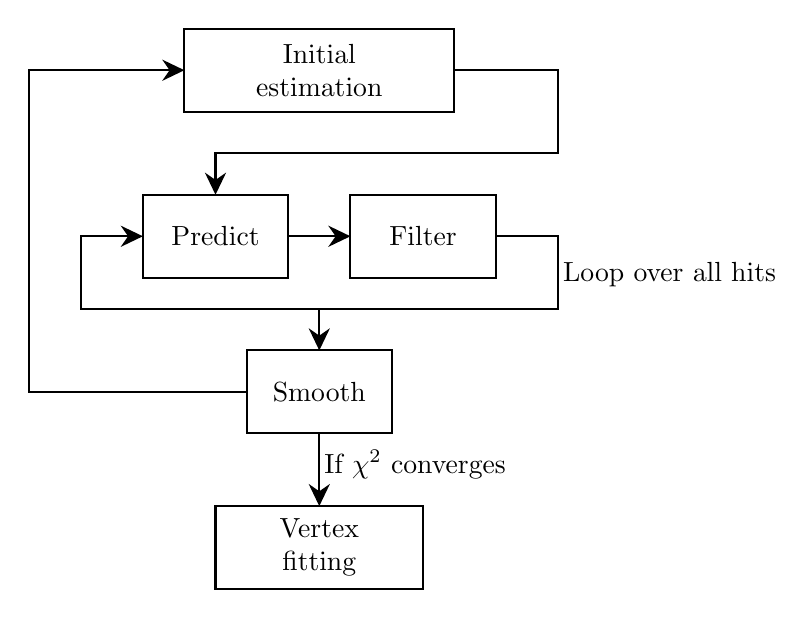
\begin{tikzpicture}[x=0.75pt,y=0.75pt,yscale=-1,xscale=1]
%uncomment if require: \path (0,283); %set diagram left start at 0, and has height of 283

%Shape: Rectangle [id:dp7390398638498927] 
\draw   (82,5) -- (212,5) -- (212,45) -- (82,45) -- cycle ;
%Shape: Rectangle [id:dp34828939700720296] 
\draw   (62,85) -- (132,85) -- (132,125) -- (62,125) -- cycle ;
%Shape: Rectangle [id:dp3361688102903969] 
\draw   (162,85) -- (232,85) -- (232,125) -- (162,125) -- cycle ;
%Shape: Rectangle [id:dp2789689137035454] 
\draw   (112,160) -- (182,160) -- (182,200) -- (112,200) -- cycle ;
%Shape: Rectangle [id:dp11930891141084887] 
\draw   (97,235) -- (197,235) -- (197,275) -- (97,275) -- cycle ;
%Straight Lines [id:da7007059310002837] 
\draw    (212,25) -- (262,25) -- (262,65) -- (97,65) -- (97,82) ;
\draw [shift={(97,85)}, rotate = 270] [fill={rgb, 255:red, 0; green, 0; blue, 0 }  ][line width=0.08]  [draw opacity=0] (10.72,-5.15) -- (0,0) -- (10.72,5.15) -- (7.12,0) -- cycle    ;
%Straight Lines [id:da2722584589858923] 
\draw    (132,105) -- (159,105) ;
\draw [shift={(162,105)}, rotate = 180] [fill={rgb, 255:red, 0; green, 0; blue, 0 }  ][line width=0.08]  [draw opacity=0] (10.72,-5.15) -- (0,0) -- (10.72,5.15) -- (7.12,0) -- cycle    ;
%Straight Lines [id:da9533508004433134] 
\draw    (232,105) -- (262,105) -- (262,140) -- (32,140) -- (32,105) -- (59,105) ;
\draw [shift={(62,105)}, rotate = 180] [fill={rgb, 255:red, 0; green, 0; blue, 0 }  ][line width=0.08]  [draw opacity=0] (10.72,-5.15) -- (0,0) -- (10.72,5.15) -- (7.12,0) -- cycle    ;
%Straight Lines [id:da15517526584615415] 
\draw    (147,140) -- (147,157) ;
\draw [shift={(147,160)}, rotate = 270] [fill={rgb, 255:red, 0; green, 0; blue, 0 }  ][line width=0.08]  [draw opacity=0] (10.72,-5.15) -- (0,0) -- (10.72,5.15) -- (7.12,0) -- cycle    ;
%Straight Lines [id:da35943866272840874] 
\draw    (112,180) -- (7,180) -- (7,25) -- (79,25) ;
\draw [shift={(82,25)}, rotate = 180] [fill={rgb, 255:red, 0; green, 0; blue, 0 }  ][line width=0.08]  [draw opacity=0] (10.72,-5.15) -- (0,0) -- (10.72,5.15) -- (7.12,0) -- cycle    ;
%Straight Lines [id:da688360676140826] 
\draw    (147,200) -- (147,232) ;
\draw [shift={(147,235)}, rotate = 270] [fill={rgb, 255:red, 0; green, 0; blue, 0 }  ][line width=0.08]  [draw opacity=0] (10.72,-5.15) -- (0,0) -- (10.72,5.15) -- (7.12,0) -- cycle    ;

% Text Node
\draw (147,25) node   [align=left] {\begin{minipage}[lt]{72.76pt}\setlength\topsep{0pt}
\begin{center}
Initial estimation
\end{center}

\end{minipage}};
% Text Node
\draw (97,105) node   [align=left] {\begin{minipage}[lt]{34pt}\setlength\topsep{0pt}
\begin{center}
Predict
\end{center}

\end{minipage}};
% Text Node
\draw (197,105) node   [align=left] {\begin{minipage}[lt]{24.48pt}\setlength\topsep{0pt}
\begin{center}
Filter
\end{center}

\end{minipage}};
% Text Node
\draw (147,180) node   [align=left] {\begin{minipage}[lt]{37.4pt}\setlength\topsep{0pt}
\begin{center}
Smooth
\end{center}

\end{minipage}};
% Text Node
\draw (147,255) node   [align=left] {\begin{minipage}[lt]{55.76pt}\setlength\topsep{0pt}
\begin{center}
Vertex fitting
\end{center}

\end{minipage}};
% Text Node
\draw (263,116) node [anchor=north west][inner sep=0.75pt]   [align=left] {Loop over all hits};
% Text Node
\draw (148,215) node [anchor=west] [inner sep=0.75pt]   [align=left] {If $\displaystyle \chi ^{2}$ converges};


\end{tikzpicture}
